\documentclass{mwart}
\usepackage{geometry}
\geometry{legalpaper, portrait, margin=1.5in}
\usepackage{tasks} %supposedly better than multicol pack.
\usepackage{multicol} %allows multicolumn itemize
\usepackage{enumitem} %allows [label={}] \alph* \Alph* \roman*
\usepackage[colorinlistoftodos]{todonotes}
\usepackage{titling}
\usepackage{amssymb} %allows \mathbb{R}
\usepackage{amsthm} %allows no theorems numbering
\usepackage[leqno]{amsmath}
\usepackage{graphicx,color}
\usepackage{colortbl}
%\usepackage[usenames,dvipsnames]{xcolor}
\usepackage{tabu}%
\usepackage{longtable}
\usepackage{breqn} %allows breaking equations (use dmath)
%\usepackage[squaren,Gray]{SIunits}
\usepackage[utf8]{inputenc}
%POLSKIE ZNAKI
\usepackage{polski}
\usepackage[utf8]{inputenc}
\usepackage[export]{adjustbox}
\usepackage{subcaption}
\captionsetup{compatibility=false}
\usepackage{wrapfig}
\usepackage{graphicx} % display images
\usepackage{makecell}%To keep spacing of text in tables
\setcellgapes{4pt}%parameter for the spacing
\usepackage{enumitem}
\usepackage{booktabs}
\usepackage{makecell}
\usepackage{floatrow}
\usepackage{sidecap}
\usepackage{caption}
\usepackage{subcaption}
\usepackage{hyperref}

\usepackage{etoolbox} %changes font to default in theorems
\setlength{\textheight}{24cm}

\makeatletter
\patchcmd{\@begintheorem}{\itshape}{}{}{}
\patchcmd{\@opargbegintheorem}{\itshape}{}{}{}
\makeatother

\theoremstyle{definition}
%prevents equations from breaking
%\relpenalty=10000
%\binoppenalty=10000

%ładne przerwy między wektorami w macierzach
\newcommand{\matsp}{\hspace*{1mm} | \hspace*{1mm}}
% symbol +/-
\newcommand{\rpm}{\raisebox{.2ex}{$\scriptstyle\pm$}}

\settasks{counter-format=(tsk[1])}

\title{Pracownia z analizy numerycznej \\
	\large Sprawozdanie do zadania P3.4.}

\author{Jan Sierpina, 291116 \\
	Oskar Tołkacz, 291583}

\date{Wrocław, \today}

\newtheorem{Def}{Definicja}
\newtheorem{Uw}{Uwaga}
\newtheorem{Tw}{Twierdzenie}
\newtheorem{Dd}{Dowód}

\begin{document}

\maketitle

\tableofcontents


\section{Wstęp}
Przeskalowywanie obrazu to jeden z podstawowych problemów w grafice komputerowej. Zapotrzebowanie na algorytmy zmieniające wymiary zdjęcia pojawia się najczęściej, gdy chcemy dany obraz powiększyć lub po prostu dopasować do określonych rozmiarów. Zadanie to nie ma jednego, optymalnego rozwiązania. Dobór odpowiedniego algorytmu zależy od tego, jaki efekt chcemy osiągnąć. Jedne z podejść powodują
wygładzanie krawędzi, inne z kolei ich mocne wyostrzanie. Profesjonalne programy obróbki obrazów dostarczają najczęściej co najmniej kilku metod skalowania. W niniejszej pracy przeanalizujemy trzy metody zmiany rozdzielczości obrazu: metodę najbliższego sąsiedztwa, metodę wykorzystującą funkcję sklejaną pierwszego stopnia i naturalną funkcję sklejaną trzeciego stopnia. Otrzymane rezultaty porównamy z edytorem graficznym GIMP.

\section{Stosowane metody}
Pośród najczęściej stosowanych metod są między innymi:
\begin{itemize}
\item Najbliższego sąsiedztwa
\item Interpolacja funkcją sklejaną pierwszego stopnia
\item Dwuliniowa - rozszerzenie metody interpolacji funkcją sklejaną pierwszego stopnia
\item Interpolacja funkcją sklejaną sześcienną
\item Interpolacja dwusześcienna - rozszerzenie interpolacji sześciennej. Jest to algorytm domyślnie stosowany przez program Adobe Photoshop.
\end{itemize}

\section{Metoda}
\label{sec:metoda}
Problem polega przekształceniu obrazu danego jako macierz $P$ o wymiarach $M_x$ na $M_y$, na macierz o wymiarach $N_x$ na $N_y$. Wartości pól macierzy $P$ odpowiadają wartości koloru poszczególnych pikseli. W przypadku wszystkich trzech stosowanych przez nas metod, zmiana szerokości i wysokości będzie wykonywana niezależnie. Co więcej, do obliczenia wartości koloru piksela o współrzędnych $x$, $y$, w przypadku zmiany szerokości, korzystać będziemy jedynie z wartości wiersza $x$ macierzy $P$, a w przypadku zmiany wysokości z kolumny $y$. Dlatego dla uproszczenia, algorytm opiszemy tylko w przypadku zmiany obrazu o wymiarach $M$ na 1, na obraz o wymiarach $N$ na 1. Taki algorytm łatwo rozszerzyć do ogólnego przypadku. \\
\indent Obraz będziemy traktować jako ciąg wartości kolorów $K(p)$ w punktach $p = 1, 2, \dots M$. Zmiana rozmiaru polega na wyznaczeniu wartości koloru $K$ w punktach $p_i = 1 +(i-1)\dfrac{M-1}{N-1}$, $(i = 1, 2, \dots , N)$.

\subsection{Metoda najbliższego sąsiedztwa}
W metodzie najbliższego sąsiedztwa przyjmujemy $K(p_i) := K(round(p_i))$. Daje to efekt "rozciągania" pikseli. 

\subsection{Funkcja sklejana pierwszegi stopnia}
W tej metodzie konstruujemy funkcję sklejaną $S$ pierwszego stopnia, taką że $S(t_i) = K(t_i)$ dla $i = 1, 2, \dots, M$, a następnie przyjmujemy $K(p_i) := S(p_i)$ $(i = 1, 2, \dots, N)$. Funkcja sklejana daje efekt płynnego przejścia pomiędzy kolorami pikseli, przez co obraz wydaje się lekko rozmazany.

\subsection{Naturalna funkcja sklejana trzeciego stopnia}
Polega na skonstruowaniu funkcji sklejanej $S$ trzeciego stopnia, takiej że $S(t_i) = K(t_i)$ dla $i = 1, 2, \dots, M$, a następnie przyjmujemy $K(p_i) := S(p_i)$ $(i = 1, 2, \dots, N)$. Ta metoda daje lepsze rezultaty od funkcji sklejanej pierwszego stopnia,
jednak wymaga większej ilości obliczeń.

\section{Porównanie wizualne}
\subsection{Powiększanie obrazu}

W przypadku powiększania zdjęć najlepsze efekty wizualne daje naturalna funkcja sklejana trzeciego stopnia, jednak nie widać wielkiej różnicy między nią, a funkcją pierwszego stopnia. Metoda najbliższego sąsiedztwa zdecydowanie pogarsza jakość obrazu, sprawiając wrażenie niskiej rozdzielczości poprzez zwykłe "rozciąganie" pikseli.

\begin{figure}[h!]
\floatbox[{\capbeside\thisfloatsetup{capbesideposition={right,top}}}]{figure}[\FBwidth]
{\caption*{Oryginalny obraz \\ O rozdzielczości 100 x 100 pikseli \\ Poniżej przedstawiono obrazy uzyskane przy skalowaniu go do rozdzielczości 250 x 250 pikseli.}\label{aa}}
{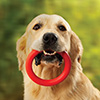
\includegraphics{dog}}
\end{figure}

\begin{figure}[h!]
\floatbox[{\capbeside\thisfloatsetup{capbesideposition={right,top}}}]{figure}[\FBwidth]
{\caption*{Obraz przeskalowany metodą najbliższego sąsiedztwa \\ Piksele wydają się być "rozciągnięte", a obraz słabej jakości.}\label{aa}}
{\includegraphics{neighbour_dog}}
\end{figure}

\begin{figure}[h!]
\floatbox[{\capbeside\thisfloatsetup{capbesideposition={right,top}}}]{figure}[\FBwidth]
{\caption*{Obraz przeskalowany funkcją sklejaną pierwszego stopnia \\ Obraz jest nieco nieostry, przejścia między kolorami są płynne i przez to rozmazane.}\label{aa}}
{\includegraphics{spline_dog}}
\end{figure}

\begin{figure}[h!]
\floatbox[{\capbeside\thisfloatsetup{capbesideposition={right,top}}}]{figure}[\FBwidth]
{\caption*{Obraz przeskalowany naturalną funkcją sklejaną trzeciego stopnia \\ Obraz jest lekko rozmazany, jednak mniej niż w przypadku funkcji sklejanej pierwszego stopnia. }\label{aa}}
{\includegraphics{spline3_dog}}
\end{figure}

%%%%%%%%%%%%%%%%%%%%%%%%%%%%%%%%%%%% CAT %%%%%%%%%%%%%%%%%%%%%%%%%%%%%%%%%
\clearpage
\subsection{Zmniejszanie obrazu}
Przy zmniejszaniu rozmiaru zdjęcia metoda najbliższego sąsiedztwa sprawia wrażenie "strzępienia obrazu". Tworzy ona obraz wybierając poszczególne piksele z obrazu, przez co małe fragmenty obrazu mogą w ogóle zniknąć. W przypadku funkcji sklejanych nie widać znaczącej utraty jakości.

\begin{figure}[h!]
	\centering
	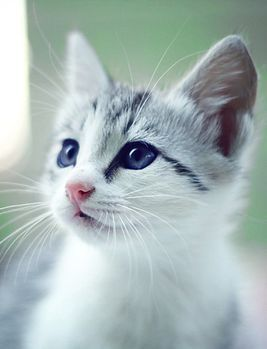
\includegraphics[width=0.7\linewidth]{cat}
	\caption*{Oryginalny obraz o rodzielczości 267 x 349 pikseli. Ponieżej przedstawiono obrazy uzyskane przy skalowaniu go do rozdzielczości 133 x 174 pikseli.}
	\label{fig:cat}
\end{figure}

\clearpage

\begin{figure}[h!]
\floatbox[{\capbeside\thisfloatsetup{capbesideposition={right,top}}}]{figure}[\FBwidth]
{\caption*{Obraz przeskalowany metodą najbliższego sąsiedztwa \\ Obraz jest bardzo "postrzępiony". Efekt ten widać szczególnie na wąsach kota. }\label{aa}}
{\includegraphics{neighbour_cat}}
\end{figure}

\begin{figure}[h!]
\floatbox[{\capbeside\thisfloatsetup{capbesideposition={right,top}}}]{figure}[\FBwidth]
{\caption*{Obraz przeskalowany funkcją sklejaną pierwszego stopnia \\ Utrata jakości jest dużo mniej widoczna, nie ma tak mocnego efektu "postrzępienia" obrazu.}\label{aa}}
{\includegraphics{spline_cat}}
\end{figure}

\begin{figure}[h!]
\floatbox[{\capbeside\thisfloatsetup{capbesideposition={right,top}}}]{figure}[\FBwidth]
{\caption*{Obraz przeskalowany naturalną funkcją sklejaną trzeciego stopnia}\label{aa}}
{\includegraphics{spline3_cat}}
\end{figure}

%%%%%%%%%%%%%%%%%%%%%%%%%%%%%%%%%%%% RESCALE %%%%%%%%%%%%%%%%%%%%%%%%%%%%%%%%%

\clearpage
\subsection{Powiększanie figur i tesktu}

\begin{figure}[h!]
\floatbox[{\capbeside\thisfloatsetup{capbesideposition={right,top}}}]{figure}[\FBwidth]
{\caption*{Oryginalny obraz \\ O rozdzielczości 80 x 30 pikseli \\ Poniżej przedstawiono obrazy uzyskane przy skalowaniu go do rozdzielczości 200 x 75 pikseli.}\label{aa}}
{\includegraphics{rescale}}
\end{figure}

\begin{figure}[h!]
\floatbox[{\capbeside\thisfloatsetup{capbesideposition={right,top}}}]{figure}[\FBwidth]
{\caption*{Obraz przeskalowany metodą najbliższego sąsiedztwa \\ Wyraźnie widać krawędzie tekstu. Widoczne są też pojedyncze piksele. }\label{aa}}
{\includegraphics{neighbour_rescale}}
\end{figure}

\begin{figure}[h!]
\floatbox[{\capbeside\thisfloatsetup{capbesideposition={right,top}}}]{figure}[\FBwidth]
{\caption*{Obraz przeskalowany funkcją sklejaną pierwszego stopnia \\ Teskt jest zdecydowanie niewyraźny.}\label{aa}}
{\includegraphics{spline_rescale}}
\end{figure}

\begin{figure}[h!]
\floatbox[{\capbeside\thisfloatsetup{capbesideposition={right,top}}}]{figure}[\FBwidth]
{\caption*{Obraz przeskalowany naturalną funkcją sklejaną trzeciego stopnia \\ Tekst jest niewyraźny, jednak widocznie lepszy niż w przypadku funkji sklejanej pierwszego stopnia.}\label{aa}}
{\includegraphics{spline3_rescale}}
\end{figure}
W przypadku tekstu i figur, często najlepsze wizualnie efekty osiągniemy za pomocą metody najbliższego sąsiedztwa. Pozostałe metody sprawiają, że krawędzie stają się rozmyte, co w przypadku obrazów dwukolorowych lub po prostu obrazów o mocnych kontrastach, może okazać się niepożądanym efektem. Przykładowo litera 'l', czyli prostokąt, w słowie Rescale po przeskalowaniu nadal pozostała idealnym prostokątem.

\clearpage
\section{Porównanie czasów}

Wykonaliśmy przeskalowania o skalach od 0,1 do 2,0 na 99 obrazach, a następnie zsumowaliśmy czasy dla kolejnych wartości skali. Poniżej przedstawiamy wykres zależności czasu wykonania programu w sekundach od skali przekształcenia w obu wymiarach. 
\begin{figure}[!h]
	\includegraphics[scale=0.5]{plot}
	\caption*{}
\end{figure}
Widzimy, że metoda najbliższego sąsiedztwa jest zdecydowanie najszybsza. Czas wykonania rośnie najszybciej dla metod wykorzystujących funkcje sklejane. Oczywiście metoda wykorzystująca funkcję sklejaną trzeciego stopnia jest najwolniejsza, ale też daje zazwyczaj najlepsze rezultaty.

\section{Inne ciekawe własności}
W następnych paragrafach przedstawimy efekt działania danego algorytmu na obrazach najpierw je powiększająć, a następnie zmniejszając, lub na odwrót. W celu badania różnic pomiędzy dwoma obrazami tych samych rozmiarów, wprowadziliśmy funkcję, którą będziemy nazywać normą obrazu. Dla obrazu o rozdzielczości $M_x$ na $M_y$ wyrażonego przez funkcję koloru $K$, jego norma to:
$$norm(K) := \dfrac{\sum_{i=1}^{M_x} \sum_{j=1}^{M_y} colorsAvg(K(i,j))}{M_x * M_y}$$
gdzie z kolei funkcja $colorsAvg$ to średnia ważona intensywności koloru czerwonego, zielonego i niebieskiego, gdzie intensywność jest wyrażona przez liczbę z przedziału $[0, 1]$. Funkcja $colorsAvg$ przyjmuje wartości od 0 do 1, gdzie 0 oznacza piksel czarny (zupełny brak koloru) a 1 piksel biały. Łatwo więc zauważyć, że funkcja $norm$ również przyjmuje wartości od 0 do 1.
Aby badać różnicę pomiędzy obrazami musimy jeszcze zdefiniować "obraz różnicy":
$$K(i, j) := |K^{(2)}(i,j) - K^{(1)}(i,j)| $$
gdzie $K$ to kolor "obrazu różnicy", a $K^{(1)}$ i $K^{(2)}$ to kolory danych obrazów. Teraz widać, że gdy norma obrazu różnicy jest równa 0, oznacza to że dwa obrazy są identyczne. Im większa norma obrazu różnicy, tym więcej dane obrazy powinny się różnić wizualnie.

\begin{figure}[!h]
  \begin{subfigure}[b]{0.4\textwidth}
    \includegraphics{spline_dog}
    \label{fig:f1}
  \end{subfigure}
  \hfill
  \begin{subfigure}[b]{0.49\textwidth}
    \includegraphics{neighbour_dog}
    \label{fig:f2}
  \end{subfigure}
  \caption*{Norma obrazu różnicy tych zdjęć wynosi 0.018}
\end{figure}

\subsection{Zwiększanie i zmniejszanie}
Zbadaliśmy wpływ zwiększenia, a następnie zmniejszenia obrazu do początkowych rozmiarów, na utratę jakości. Przetestowaliśmy nasze trzy algorytmy na 100 różnych obrazkach, przyjmując losowy współczynnik skalowania. Zawsze był on jednak większy od 1, tak aby obraz najpierw powiększyć, a później z powrotem zmniejszyć. Tworzyliśmy obraz różnicy oryginalnego obrazu i drugiego, będącego wynikiem dwukrotnego skalowania. Poniżej zapisane są maksymalne wartości norm różnicy obrazów, które uzyskaliśmy. \\

\begin{tabular}{|r|c|}
  \hline 
  Algorytm & Maksymalna norma różnicy\\
  \hline
  Najbliższe sąsiedztwo & 0.0 \\
  \hline
  Funkcja sklejana pierwszego stopnia & 0.0235 \\
  \hline
  Naturalna funkcja sklejana trzeciego stopnia &  0.0160 \\
  \hline
\end{tabular}

\vspace{5mm}

 W przypadku tak małych wartości norm, jak te uzyskane, niewiele jesteśmy w stanie powiedzieć o tym czy różnica wizualna będzie dostrzegalna. Ciekawym natomiast faktem jest uzyskany zerowy wynik dla metody najbliższego sąsiedztwa. Okazuje się przy powiększaniu obrazka tą metodą, a następnie pomniejszaniu go z powrotem do początkowych rozmiarów, uzyskujemy dokładnie ten sam obraz. To znaczy, że w wyniku dowolnej liczby takich skalowań nie utracimy jakości obrazu. Dowód tego twierdzenia przedstawiamy poniżej. \\
\indent Przyjmujemy definicje podane w paragrafie \hyperref[sec:metoda]{[3]}. Będziemy skalować obraz o rozmiarach $M$ na 1 do rozmiarów $N$ na 1 i z powrotem, gdzie $M<N$. Niech $K$ oznacza obraz przed skalowaniem, $K^{(1)}$ po powiększeniu, $K^{(2)}$ po pomniejszeniu do pierwotnych rozmiarów. Niech $i$ oznacza pewien dowolny punkt obrazu $K^{(2)}$, $i \in (1,\dots,M)$. \\
Pokażemy, że $K^{(2)}(i)=K(i)$. \\
\textbf{Dowód.}
Skalując obraz z $K^{(1)}$ do $K^{(2)}$ mamy:
$$p_i = 1 + (i-1)\frac{N-1}{M-1}$$
Niech $j := round(p_i)$. Wtedy $K^{(2)}(i)=K^{(1)}(j)$. Przy skalowaniu $K$ do $K^{(1)}$ dla punktu $j$ mamy:
$$p_j = 1 + (j-1)\frac{M-1}{N-1}$$
Czyli $K^{(1)}(j) = K(round(p_j))$. Dla tezy wystarczy pokazać $i = round(p_j)$ ($round(p_j)$ to pewien punkt od którego zaczęliśmy skalowanie, a skończyliśmy na $i$. W rozumowaniu szliśmy od tyłu).
Wyjdziemy od tezy i dojdziemy to tożsamości. Mamy
$$round(p_j) = round(1 + (j-1)\frac{M-1}{N-1}) = round(1 + (round(p_i)-1)\frac{M-1}{N-1}) = $$
$$ = round(1 + (round[1 + (i-1)\frac{N-1}{M-1}]-1)\frac{M-1}{N-1})  = $$
$$ = 1 + round(round[(i-1)\frac{N-1}{M-1}]\frac{M-1}{N-1}) $$
Wystarczy pokazać, że: \\
\textbf{Lemat.} Dla $b>1, a>0$ zachodzi $round(round(a*b)\frac{1}{b}) = a$. \\
\textbf{Dowód.} Wystarczy pokazać, że $a-\frac{1}{2}<round(a*b)\frac{1}{b}\leq a+\frac{1}{2}$, \\
czyli $a*b-\frac{1}{2}b < round(a*b) \leq a*b + \frac{1}{2}b$, ale $b>1$ stąd mamy tezę.\\ \qed

\subsection{Kierunek przeskalowywania}
Sprawdziliśmy, czy to, w którą stronę najpierw przeskalujemy obraz - pionowo czy poziomo - ma wpływ na uzyskany rezultat. Przetestowaliśmy nasze algorytmy na 100 różnych obrazkach z różnymi współczynnikami skalowania, zarówno powiększaniem jak i pomniejszaniem. Obliczaliśmy normę obrazu różnicy, pomiędzy obrazami uzyskanymi skalując najpierw wysokość i najpierw szerokość. Poniżej zaprezentowane zostały uzyskane przez nas wyniki. \\

\begin{tabular}{|r|c|}
  \hline 
  Algorytm & Maksymalna norma różnicy\\
  \hline
  Najbliższe sąsiedztwo & 0.0 \\
  \hline
  Funkcja sklejana pierwszego stopnia & 0.00084 \\
  \hline
  Naturalna funkcja sklejana trzeciego stopnia &  0.0010 \\
  \hline
\end{tabular} \\

Widzimy, że w przypadku metody najbliższego sąsiedztwa, kierunek pierwszego skalowania nie ma znaczenia. Natomiast w przypadku funkcji sklejanych uzyskane rezultaty są różne.

\section{Porównanie z programem GIMP}
Program graficzny GIMP pozwala na korzystanie z czterech metod skalowania obrazu. Oprócz trzech metod, które zaimplementowaliśmy, w GIMPie dodatkowo znajdziemy metodę sinc (Lanczos). Używa ona funkcji $$sinc(x) = \frac{sin(x)}{x}$$ do znalezienia funkcji interpolującej wartości kolorów.

\begin{figure}[!h]
	\begin{subfigure}[b]{0.4\textwidth}
		\includegraphics{gimp_spline3_dog}
		\label{fig:f1}
	\end{subfigure}
	\hfill
	\begin{subfigure}[b]{0.49\textwidth}
		\includegraphics{spline3_dog}
		\label{fig:f2}
	\end{subfigure}
	\caption*{Metoda funkcji sklejanej trzeciego stopnia. Obraz wygenerowany w programie GIMP po lewej, po prawej zaprogramowana metoda. Jak widać obrazki są praktycznie identyczne, podobnie jest w przypadku pozostałych metod.}
\end{figure}

\begin{figure}[!h]
	\includegraphics{gimp_sinc_dog}
	\caption*{Metoda sinc(Lanczos)}
\end{figure}

Metoda Lanczosa daje obrazek, który ma bardziej wygładzone krawędzie.
\clearpage
\section{Wnioski}
Po przeprowadzeniu różnych testów dochodzimy do wniosku, że każda metoda daje obrazy o innych cechach i bardzo dużo zależy od subiektywnych odczuć obserwatora. Do różnych zastosowań najlepsze będą różne metody. Nawet metoda najbliższego sąsiedztwa może mieć zastosowanie, np. w przypadku gdy chcemy przeskalować obraz z dużą ilością ostrych krawędzi i chcemy, żeby były one nadal widoczne po przeskalowaniu. Tak może być w przypadku pixel artów. Pozostałe metody sprawiają, że obraz jest bardziej rozmyty i zazwyczaj subiektywnie wygląda lepiej. Jednak te metody wymagają większej ilości obliczeń, co może powodować, że nie będzie się nadawać do pewnych zastosowań.
\begin{thebibliography}{9}

\bibitem{blewitt}
  Przemysław Wójtowicz,
  \textit{Cyfrowe metody powiększania obrazów rastrowych},
  Politechnika Warszawska,
  2004.

\bibitem{blewitt}
  https://www.cambridgeincolour.com/tutorials/digital-photo-enlargement.htm,
Cambridge in Colour.

\end{thebibliography}

\end{document}
